\documentclass[tikz]{standalone}
\usetikzlibrary{calc}

  \usepackage[no-math]{fontspec}
  \setmainfont{TeXGyreTermes-Regular}[
       BoldFont       = TeXGyreTermes-Bold ,
       ItalicFont     = TeXGyreTermes-Italic ,
       BoldItalicFont = TeXGyreTermes-BoldItalic,
       NFSSFamily     = ntxtlf]
  \setsansfont{TeX Gyre Heros Regular}[
       Scale=.9,
       BoldFont       = TeX Gyre Heros Bold,
       ItalicFont     = TeX Gyre Heros Italic,
       BoldItalicFont = TeX Gyre Heros BoldItalic]
  \setmonofont[StylisticSet={1,3},Scale=.9]{inconsolata}
  \usepackage{newtxmath}
\begin{document}

\definecolor{Maroon}{cmyk}{0, 0.87, 0.68, 0.32}
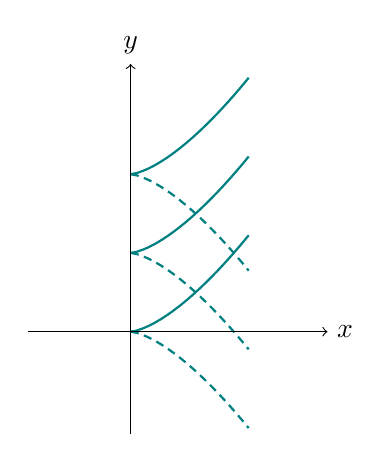
\begin{tikzpicture}
\def\xmax{2} \def\xmin{-0.8}
\def\ymax{2.9} \def\ymin{-0.8}

% Plot a particular solution passing through y0
\draw[color=teal, variable=\t, thick] plot[domain=0:1.5, samples=20] ({\t},{2/3 * \t^(3/2)+2});
\draw[color=teal, variable=\t, densely dashed,thick] plot[domain=0:1.5, samples=20] ({\t},{-2/3 * \t^(3/2)+2});

\draw[color=teal, variable=\t,thick] plot[domain=0:1.5, samples=20] ({\t},{2/3 * \t^(3/2)+1});
\draw[color=teal, variable=\t, densely dashed,thick] plot[domain=0:1.5, samples=20] ({\t},{-2/3 * \t^(3/2)+1});

\draw[color=teal, variable=\t,thick] plot[domain=0:1.5, samples=20] ({\t},{2/3 * \t^(3/2)});
\draw[color=teal, variable=\t, densely dashed,thick] plot[domain=0:1.5, samples=20] ({\t},{-2/3 * \t^(3/2)});

\draw[->] (\xmin-.5,0)--(\xmax+.5,0) node[right] {$x$};
\draw[->] (0,\ymin-.5)--(0,\ymax+.5) node[above] {$y$};
\end{tikzpicture}
\end{document}